\documentclass[twoside]{article}
\usepackage{listings}
\usepackage{color}
\usepackage{verbatim}
\usepackage{amsmath}
\definecolor{dkgreen}{rgb}{0,0.6,0}
\definecolor{gray}{rgb}{0.5,0.5,0.5}
\definecolor{mauve}{rgb}{0.58,0,0.82}
\usepackage{amssymb}
\usepackage{amsthm}
\usepackage{thmtools}
\usepackage{graphicx}


% \lstset{frame=tb,
%   language=Java,
%   aboveskip=3mm,
%   belowskip=3mm,
%   showstringspaces=false,
%   columns=flexible,
%   basicstyle={\small\ttfamily},
%   numbers=none,
%   numberstyle=\tiny\color{gray},
%   keywordstyle=\color{blue},
%   commentstyle=\color{dkgreen},
%   stringstyle=\color{mauve},
%   breaklines=true,
%   breakatwhitespace=true
%   tabsize=3
% }

\lstset{
  aboveskip=0mm,
  belowskip=0mm,
  showstringspaces=false,
  columns=flexible,
  basicstyle={\small\ttfamily},
  numbers=none,
  numberstyle=\tiny\color{gray},
  keywordstyle=\color{blue},
  commentstyle=\color{dkgreen},
  stringstyle=\color{mauve},
  breaklines=true,
  breakatwhitespace=true
  tabsize=3
}

%%%%%%%%%%%%%%%%%%%%%%%%%%%%%%%%%%%%%%%%%
% Stylish Colored Title Page 
% LaTeX Template
% Version 1.0 (27/12/12)
%
% This template has been downloaded from:
% http://www.LaTeXTemplates.com
%
% Original author:
% Peter Wilson (herries.press@earthlink.net)
%
% License:
% CC BY-NC-SA 3.0 (http://creativecommons.org/licenses/by-nc-sa/3.0/)
% 
% Instructions for using this template:
% This title page compiles as is. If you wish to include this title page in 
% another document, you will need to copy everything before 
% \begin{document} into the preamble of your document. The title page is
% then included using \titleBC within your document.
%
%%%%%%%%%%%%%%%%%%%%%%%%%%%%%%%%%%%%%%%%%

%----------------------------------------------------------------------------------------
%	PACKAGES AND OTHER DOCUMENT CONFIGURATIONS
%----------------------------------------------------------------------------------------


\usepackage[svgnames]{xcolor} % Required to specify font color

\newcommand*{\plogo}{\fbox{$\mathcal{PL}$}} % Generic publisher logo


%----------------------------------------------------------------------------------------
%	TITLE PAGE
%----------------------------------------------------------------------------------------

\newcommand*{\rotrt}[1]{\rotatebox{90}{#1}} % Command to rotate right 90 degrees
\newcommand*{\rotlft}[1]{\rotatebox{-90}{#1}} % Command to rotate left 90 degrees
\def \a {NavyBlue}
\def \b {Magenta}
\def \c {Purple}
\def \n {4}
\def \prof {Prof. Prakash Panangaden}
\def \courseTitle {Comp 250}
\def \date {Monday October 20, 2013}
\newcommand*{\titleBC}[4]{\begingroup % Create the command for including the title page in the document
\centering % Center all text

\def\CP{\textit{\Huge Assignment #1}} % Title

%\settowidth{\unitlength}{\CP} % Set the width of the curly brackets to the width of the title
%{\color{LightGoldenrod}\resizebox*{\unitlength}{\baselineskip}{\rotrt{$\}$}}} \\[\baselineskip] % Print top curly bracket
%\textcolor{Sienna}{\CP} \\[\baselineskip] % Print title
%{\color{RosyBrown}\Large for Prof. Sergey Norin} \\ % Tagline or further description
%{\color{LightGoldenrod}\resizebox*{\unitlength}{\baselineskip}{\rotlft{$\}$}}} % Print bottom curly bracket


\settowidth{\unitlength}{\CP} % Set the width of the curly brackets to the width of the title
{\color{\a}\resizebox*{\unitlength}{\baselineskip}{\rotrt{$\}$}}} \\[\baselineskip] % Print top curly bracket
\textcolor{\b}{\CP} {\color{\a}{\\ #2}} \\[\baselineskip] % Print title
{\color{\c}\Large for #3} \\ % Tagline or further description
{\color{\a}\resizebox*{\unitlength}{\baselineskip}{\rotlft{$\}$}}} % Print bottom curly bracket

%Default are LightGoldenrod / Sienna / RosyBrown / LightGoldenrod

%\vfill % Whitespace between the title and the author name
\vspace*{\fill}
{\Large\textbf{by Alan Do-Omri\\260532985}}\\ % Author name
\vspace*{\fill}
#4

\endgroup}
\linespread{1.05}
\usepackage{lipsum}
\usepackage{multicol}
\usepackage{alltt}
\usepackage[margin=1in]{geometry}
\usepackage{mathtools}
% \usepackage{subcaption}
\usepackage{hyperref}
\usepackage{paralist}
\usepackage{float}
\usepackage{microtype}
\usepackage{abstract}
\usepackage[utf8]{inputenc}
\usepackage[numbers]{natbib}
\usepackage{graphicx}
\renewcommand{\abstractnamefont}{\large\bfseries} % Set the "Abstract" text to bold
\renewcommand{\abstracttextfont}{\normalfont\itshape} % Set the abstract itself to small italic text
\usepackage{lettrine}
\usepackage{tabulary}
\usepackage{import}
\usepackage{enumitem}
\usepackage{paralist}
\usepackage{pgf}
\usepackage{caption}
\usepackage{subcaption}
\usepackage{booktabs}
\newenvironment{Figure}
  {\par\medskip\noindent\minipage{\linewidth}}
  {\endminipage\par\medskip}

\usepackage{titlesec} % Allows customization of titles
%\renewcommand\thesection{\Roman{section}} % Roman numerals for the sections
%\renewcommand\thesubsection{\Roman{subsection}} % Roman numerals for subsections
\titleformat{\section}[block]{\Large\scshape\centering\bfseries}{\thesection.}{1em}{} % Change the look of the section titles
\titleformat{\subsection}[block]{\large\bfseries}{\thesubsection.}{1em}{} % Change the look of the section titles

\usepackage{fancyhdr} % Headers and footers
\pagestyle{fancy} % All pages have headers and footers
\fancyhead{} % Blank out the default header
\fancyfoot{} % Blank out the default footer
\fancyhead[C]{Virus Classification from Transmission Electron Microscopy $\bullet$ Fall 2015} % Custom header text
\fancyfoot[RO,LE]{\thepage} % Custom footer text

\title{\fontsize{18pt}{10pt}\textbf{Classifiying Transmission Electron Microscopy Virus Textures}} % Article title

% \author{
% \large{Alan Do-Omri}\\[2mm] % Your name
% \normalsize McGill University \\ % Your institution
% \normalsize \href{mailto:alan.do-omri@mail.mcgill.ca}{alan.do-omri@mail.mcgill.ca}}

\author{
\large{Alan Do-Omri}\\[2mm] 
\normalsize 260532985 \\ 
\and 
\large{Kian Kenyon-Dean}\\[2mm]
\normalsize 260564475 \\
\and
\large{Genevieve Fried}\\[2mm]
\normalsize 260564432 \\
}


\begin{document}

\maketitle

\begin{abstract}
On a daily basis doctors are tasked with determining the identity of viruses from blood samples. Even with advanced microscopy techniques, viruses can be difficult to discern by the expert human eye. Unfortunately, Misclassifying can have grave implications, not only for the patients in question but also for those who come into contact with him or her. Fortunately, virus classification is an image classification problem, and machine learning methods present exceedingly high accuracy rates for image classification tasks and don't require expert knowledge to do so. Here we present a successful application of Convolutional Neural Networks (CNN) to the problem of virus classification. Using the Virus Texture Dataset from Uppsala University, we classify viruses samples into one of 15 categories and compare its performance to previous work done on the same task.

\end{abstract} 
\vspace{0.5cm}

\begin{multicols}{2}
\section{Introduction}
Identifying viral pathogens, existing and emerging, is a critical priority for public health. Current diagnostic methods include direct examination of a speciman by an trained medical professional using Electron Microscopy methods. Unfortunately, even with magnification techniques it can be difficult for doctors to identify specific viral types. 

On the other hand, automatic classification methods in machine learning have proven quite successful at image classification. In particular, research employing neural networks has reshaped image classification in recent years \citet{Juergen_2015}. Specifically, Max Pooling Convolutional Neural Networks have set the bar at it's highest for an array of tasks, including the multi-digit number recognition in Google Street View images, reCAPTCHA box classification \citet{DBLP:journals/corr/GoodfellowBIAS13}, and ImageNet classification \citet{NIPS2012_4824}. 

The high degree of accuracy obtained with these automated methods is highly desirable for a problem like virus classification. In the desire to determine a model that accurately predicts known virus types, we treat the virus classification as an image classification problem. We use the Virus Texture Dataset from Uppsala University containing images of fifteen different virus types, which we extend through random rotations to enlarge our dataset. 

We experiment with an array of machine learning classifiers, including Support Vector Machines with linear and radial basis function kernels, Gaussian Naive Bayes, Logistic Regression, Random Forest Trees and Feed Forward Neural Networks with local binary pattern feature extractors. Our best results come from our Convolutional Neural Network (CNN)using max pooling, with which we classify virus samples from our dataset into one of 15 categories with an accuracy of approximately 85\%. 


\section{Problem Definition}

Our research takes place in a greater context of a desire to use machine learning classification methods to accurately classify viruses from viral sample images. This extends to both viruses which are currently known, and potentially evolved viruses like the H1N1 influenza pandemic virus in Mexico and the US in 2009, which was a modified version of known influenza strains. Convolutional Neural Networks with all the function approximation power of Neural Networks, but specifically architected for images, present a highly promising solution for computer automated virus identification, and a useful supplementation to traditional virology research. 

From our survey of the work done in virus classification, treating virus classification as an image classification problem is not common. Most researchers have used Support Vector Machines, tree modeling structures like Random Forests, and Feed Forward Neural Networks to classify and predict known and emerging viral strains through analysis of genome segments and genetic sequences \citet{work_A} \citet{work_B} \citet{work_C}. \citet{kylberg2011virus}, which we looked to for insight into feature extraction methods, use a Random Forest classifier to assess the discriminant potential of various texture measures on virus images. As far as we can tell, using a CNN is rather unprecedented for this problem. Thus we find the application of CNNs to virus classification a pertinent one that would be fruitful to explore further.

\section{Methodology}

\subsection{Feature Design and Selection Methods}
%% related work shit should actually go here
%%TODO: PUT RELATED WORKS UNDER FEATURE DESIGN

\subsubsection{Related Work}
In the work of \citet{kylberg2011virus}, texture analysis is performed on a dataset composed of 22 different  virus samples and the resulting feature vector is fed into a Random Forest classifier. The authors first compare the performance of different texture analysers, such as Local Binary Patterns, Radial Density Profile and their respective variants before proceeding to detail their results. We will briefly explain their feature extractors and results here. 
\subsection{Local Binary Pattern (LBP)}
Local Binary Pattern works such that, given an image, for each pixel $p_i$ in it we sample $n$ equally-spaced points on the circle of radius $r$ with center $p_i$ -- an example of sampling is shown in figure \ref{fig:lbp_basic} -- and construct a vector $v(p_i)$ such that its $i$th entry is a 1 if the $i$th sampled pixel has a value bigger than $p_i$ and 0 otherwise. 
\begin{Figure}
	\centering
	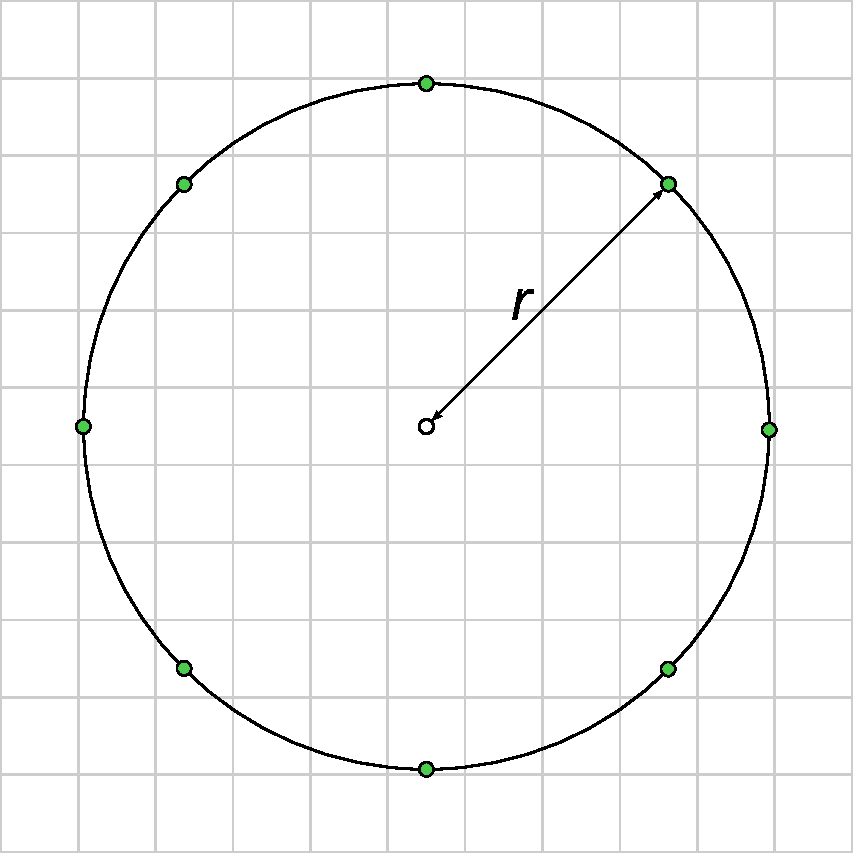
\includegraphics[width=0.5\linewidth]{images/lbp_basic.pdf}
	\captionof{figure}{Example of LBP sampling: The green points are the neighbouring sample points at distance $r$ from the central white point. In this case, we are sampling with $n=8$ neighbour points.}
	\label{fig:lbp_basic}
\end{Figure}
A sequence of 0s and 1s are constructed $v(p_i)$ to form a binary number $v_{p_i}$, hence the name. Once we have the $v_{p_i}$ for all pixels, we construct a histogram counting the number of appearances of each value $v_{p_i}$. The histogram forms the feature vector associated with the given image. \citet{kylberg2011virus} denote this feature extraction method by LBP$_{n, r}$, where $n$ is the number of sampled points and $r$ is the radius, as described above. The resulting histogram is represented in a vector of counts with $2^n$ elements. 
\paragraph{Rotational Invariant LBP} In order to reduce the size of the feature vector, \citet{kylberg2011virus} mention a modification of LBP in the following sense: instead of creating $v_{p_i}$ by interpreting the vector $v(p_i)$ and using $v_{p_i}$ as is, rotate the number $v_{p_i}$ bitwise until you get the smallest possible number. For example, the number 110 becomes 011. They name this technique the rotational invariant and denote it with LBP$^{\textnormal{ri}}_{n,r}$.
\paragraph{Uniform LBP} To further reduce the size of the histogram, Kylberg et. al also restrict the values of $v_{p_i}$ to only numbers that have 2 or less transitions from 0 to 1 or from 1 to 0, and they call this variant \emph{uniform binary patterns with at most 2 spatial transitions}, denoted LBP$^{\textnormal{u2}}_{n,r}$. For example, 01010 has 2 transitions from 0 to 1 and 2 transitions from 1 to 0 which makes 4 transitions in total. This version then LBP$^{\textnormal{u2}}_{n,r}$ does not count the number 01010. On the other hand, 00111 has only 1 transition from 0 to 1 so it is accepted. 
\par 
\paragraph{Gaussian Filtered LBP} Finally, \citet{maenpaa2003multi} talk about an extension to the LBP that is also used in the work of \citet{kylberg2011virus}, which consists of sampling neighbours about a central pixel at different radii. Instead of sampling these points equidistantly in a circle, the authors sample according to a Gaussian distribution. Figure \ref{fig:rdp} shows an example of such a sampling. \citet{kylberg2011virus} denote it as LBPF$^{\textnormal{ri}}_{n_1,r_1}$ $+$ $^{\textnormal{ri}}_{n_2,r_2}$ $+$ $\cdots$ $+$ $^{\textnormal{ri}}_{n_j,r_j}$ for the different numbers of sample points $n_1, n_2, \cdots, n_j$ and different radii distances $r_1, r_2, \cdots, r_j$.
\begin{Figure}
	\centering
	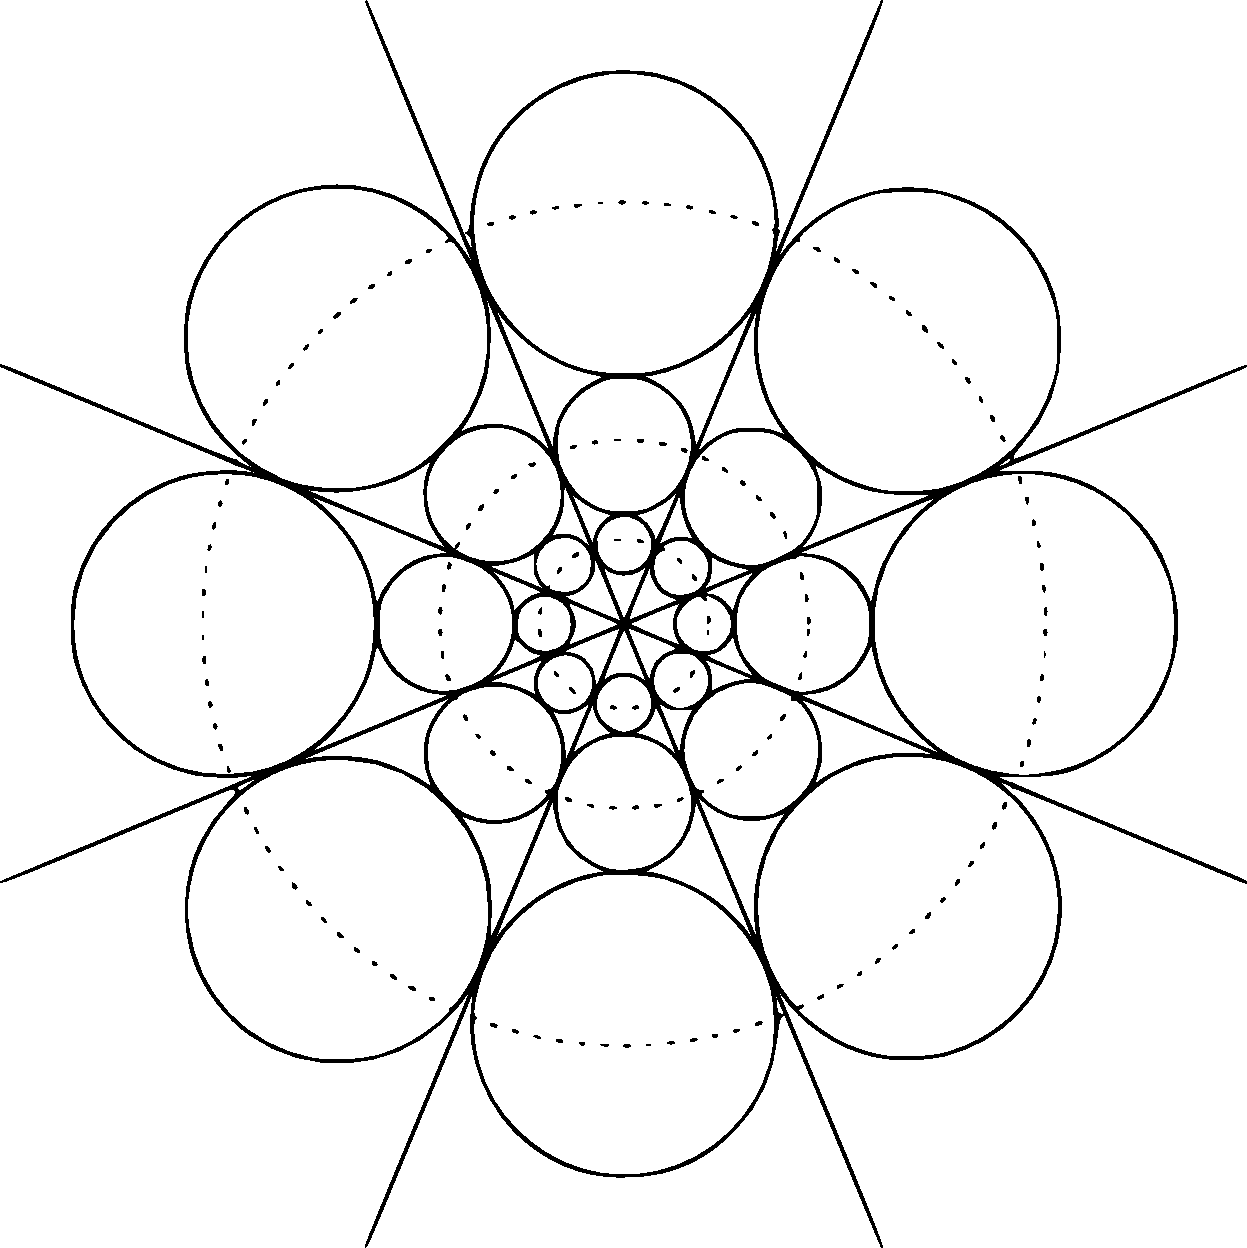
\includegraphics[width=0.5\linewidth]{images/lbpf.pdf}
	\captionof{figure}{Example of LBPF sampling: In the simple LBP, the points would be sampled at equal distances around the dotted circles for one radius as in figure \ref{fig:lbp_basic} but with this extension, the points are sampled according to a Gaussian distribution inside the solid black circles at multiple radii. In this picture, the number of neighbours also vary with the radii. This image comes from \citet{maenpaa2003multi}.}
	\label{fig:lbpf}
\end{Figure}
\subsection{Radial Density Profile (RDP)}
This method is a way to get the mean intensity in a ring around each pixel in the image. \citet{kylberg2011virus} defines the \emph{radial mean intensity $f$} around a center pixel $q_c$ as 
\[ f(q_c, r) = \frac{1}{|N|} \sum\limits_{q\in N} I(q) \]
where $I(q)$ is the pixel value for pixel $q$ and $N = \left\{ q: \Vert q-q_c \Vert_2 \in \left( r-\frac{1}{2}, r+\frac{1}{2} \right] \right\}$ is the set of pixels in a ring around $q_c$ of width 1 at distance $r$ from $q_c$. Figure \ref{fig:rdp} shows an example of what the set $N$ may look like. Following the notation from \citet{kylberg2011virus}, let $\bar{f}_{q_c}$ be the mean of the set $\{ f(q_c,i) \}_{i = 1, \cdots, n}$. Then they define the radial density profile for that pixel $q_c$ as $\textnormal{RDP}_n = \left[ f(q_c,1)-\bar{f}_{q_c}, f(q_c, 2)-\bar{f}_{q_c}, \cdots, f(q_c,n)-\bar{f}_{q_c} \right]$. 
\begin{Figure}
	\centering
	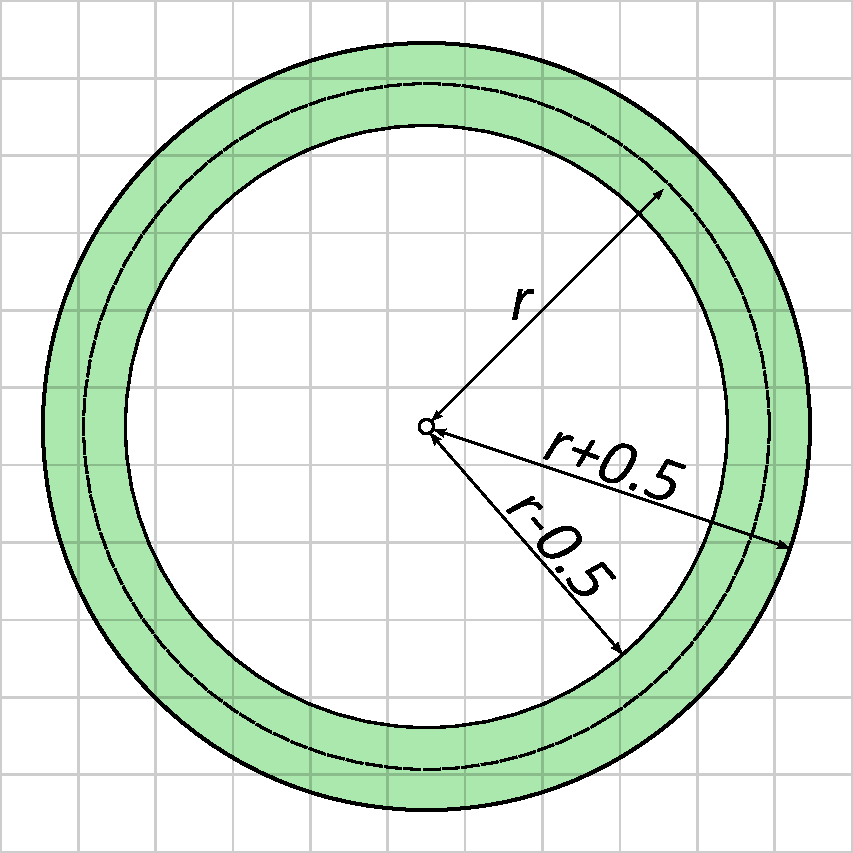
\includegraphics[width=0.5\linewidth]{images/rdp.pdf}
	\captionof{figure}{Example of RDP sampling: The green zone is the set of sampled pixels for a given radius $r$.}
	\label{fig:rdp}
\end{Figure}
\par It is not explained how the pixel features are combined to make the feature vector for the whole image but we would imagine that the feature vector for the whole image is either a concatenation of the pixel features or the concatenation of the mean of each pixel feature. 
\paragraph{Fourier RDP} One variation \citet{kylberg2011virus} introduced is applying the same RDP technique on the image after it undergoes a Fourier transform and looking at it with respect to a base $e$ logarithmic scale. They denote it with FRDP$_n$.

\subsection{Results}
\label{text:relwork_results}
The first thing to note is that \citet{kylberg2011virus} made modifications to the images' scales. In one case, one pixel in the image corresponded to 1 nanometer, they refer to that scale as \emph{fixed scale}. In the other case, the radius of the virus is set to take 20 pixels, they refer to that scale as \emph{object scale}. The classifier used was a Random forest with 100 trees (they tried up to 200 with no significant improvement with respect to 100 trees). The different textures \citet{kylberg2011virus} used were among 
\begin{compactenum}
\item LBP$^\textnormal{ri}_{8,2}$
\item LBP$^\textnormal{riu2}_{8,2}$
\item LBPF$^\textnormal{ri}_{8,1}+^\textnormal{ri}_{8,2.4}+^\textnormal{ri}_{8, 5.4}$
\item LBPF$^\textnormal{riu2}_{8,1}+^\textnormal{riu2}_{8,2.4}+^\textnormal{riu2}_{8, 5.4}$
\item RDP$_{20}$
\item FRDP$_{20}$
\end{compactenum}
All values are chosen after a grid search. Figure \ref{fig:relwork_results} shows their results with respect to the six aforementioned texture extractors and on both fixed and object scale images. They conclude that LBPF$^\textnormal{ri}_{8,1}+^\textnormal{ri}_{8,2.4}+^\textnormal{ri}_{8, 5.4}$ performed the best in fixed scale (median 21\% error) whereas FRDP$_{20}$ performed the best in object scale (median 22\% error). They also noticed that combining these two texture extractors, they could get an even better result (median 13\% error). 
\begin{figure*}
	\centering
	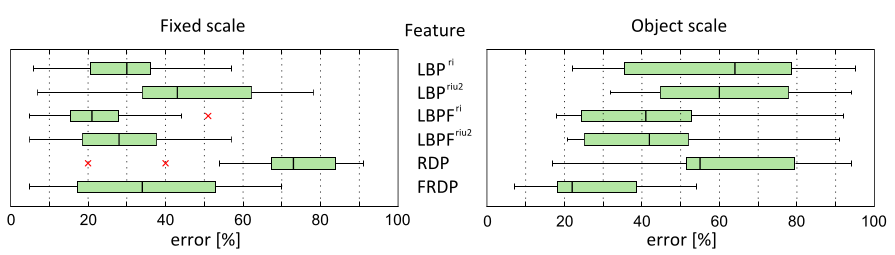
\includegraphics[width=\linewidth]{images/boxes_results.png}
	\captionof{figure}{This figure comes from \citet{kylberg2011virus}. The classification errors are shown for a Random Forest classifier using the 6 different texture extractors as described in section \ref{text:relwork_results}. The boxes' vertical lines represent the median and the red $\times$ represent outliers that are at least 1.5 times the size of the box away from it. The error bars are from the lower to the upper quartile.}
	\label{fig:relwork_results}
\end{figure*} 


\subsection{Data and Pre-Processing Methods}
\label{text:dataset}
The Virus Texture Dataset contains images (texture samples) of 15 virus types obtained through transmission electron microscopy (TEM). The texture samples are extracted using an automatic segmentation method used in \citet{JMI:JMI3556} that detects virus particles of various shapes in TEM using a series of analytical steps. Each virus class has 100 unique texture patches of size 41x41 pixels. It is a rather small dataset for the purposes of our CNN so we chose to extend it by generating twelve random rotations for each image in the dataset, producing 18,000 more images.

\section{Baseline Classification Approach}
We tested 4 different classifiers using algorithms from the scikit-learn \citet{scikit-learn} machine learning library. These baseline classifiers provide results that help to reveal the dataset's complexity. We trained and tested these classifiers over the rotated dataset. Not surprisingly, the SVM with an rbf kernel performed the best since it allows projection of the pixel feature space to a higher dimension, thus making it capable of capturing aspects of the data that cannot be observed by the other classifiers. These classifiers clearly have poor results, but they provide a good baseline understanding of the dataset, showing that the image pixel space is not easily separable and requires a stronger non-linear function approximator in order to be properly understood. See the appendix for the confusion matrices of the results.


\begin{table}
\resizebox{\textwidth}{!}{
	\begin{tabular}{llc}
	\toprule
	\multicolumn{1}{c}{\textbf{Classifier}} & \textbf{Parameters} & \textbf{F1-Accuracy} \\ \midrule
	Logistic Regression  & default         & 0.271 \\ 
	Linear 	SVM   	     & linear kernel   & 0.248 \\
	SVM                  & rbf kernel      & 0.327 \\
	Gaussian Naive Bayes & none            & 0.273 \\ \bottomrule
	\end{tabular}
}\end{table}


\section{Neural Networks Approach}
In order to establish a baseline, we combine ideas from \citet{kylberg2011virus} and ourselves by attempting to use a neural network with the LBP features. Our neural networks are built using the Lasagne and Theano \cite{Bastien-Theano-2012, bergstra+al:2010-scipy} libraries. In our experiments, we will not rescale the images and we will use LBP$_{8,2}$, an implementation given by the \emph{Mahotas} computer vision library \citet{coelho2012mahotas}. We are not scaling the images because we are later comparing to CNNs, which will not use rescaled images. The values of $8,2$ come from the best values as checked by \citet{kylberg2011virus}. \emph{Mahotas}' implementation of LBP is done so that the feature vector is of smaller dimension than the usual dimension of a histogram with $2^N$ values where $N$ is the number of sampled points. This is achieved by some optimization on their end. 
To normalize the data, we chose to divide the entire dataset by 1.1 times the maximum value of a feature in the training set in order to be more certain that no features in the normalized test set would have a value greater than 1. In all cases, we are using a learning rate of 0.005 and an L2 regularization weight of 0.0001, both arbitrarily chosen and the last layer was a 15 units softmax layer. The dataset described in section \ref{text:dataset} is shuffled and the training is done with a batch size of 16 by stochastic gradient descent. All images pertaining to the results such as the confusion matrices for the validation and testing set and the learning curves can be found in the Appendix: the first neural network results are found in figures \ref{shrine1_curves} and \ref{shrine1_mat}; the second neural network results are found in figures \ref{shrine0_curves} and \ref{shrine0_mat}; the third nerual network results are found in figures \ref{shrine2_curves} and \ref{shrine2_mat}. The table below shows the results obtained on the test set. The first column represent, in order, the number of units in each of the hidden layers. 
\subsection{Results}

\begin{tabular}{lc}
\multicolumn{1}{c}{\textbf{Hidden Layers}} & \textbf{Test Error} \\
\textbf{256 units}                         &   52.77 \%          \\
\textbf{256 and 256 units}                 &   52.22 \%          \\
\textbf{256, 128 and 64 units}             &   51.94 \%                 
\end{tabular}

\subsection{Discussion}
We had to stop the training of the one hidden layer neural network due to time constraints. We notice that the neural network with one hidden layer takes the longest time to converge whereas the one with three hidden layers took the shortest time. On the other hand, the network with three hidden layers overfitted the quickest. This is to be expected since it has many more parameters than the network with one layer. We also notice that the network with one hidden layer has the biggest error and we think this is because the network does not have enough neurons to learn properly. The three hidden layers network has too many neurons and is overfitting but we think its results can be improved by adding Gaussian noise to neurons and dropping out some of them. Nonetheless, it is still the network that gave the best results. 
\par Compared to the work of \citet{kylberg2011virus}, we can see from Figure \ref{fig:relwork_results} that the LBP$^{\textnormal{ri}}$ on fixed scale performed at about 30 \% error whereas on the object scale it performed at about 63 \%. Since we didn't perform any rescaling of the images, we expect the error to be within that interval. Finally, \emph{Mahotas}' implementation of LBP does not necessarily match the implementation of LBP$^{\textnormal{ri}}$ so this can induce some error as well. 
\end{multicols}


\section{Convolutional Neural Network Approach}
CNNs are often used in image classification tasks as they possess the power of Feed Forward Neural Networks but are specifically structured to process images efficiently. As we approached the problem of virus classification from an image classification approach, CNNs seemed a natural method to use.
Our CNN is build with the Lasagne and Theano \cite{Bastien-Theano-2012, bergstra+al:2010-scipy} libraries. Our CNNs first convolutional layer is fed by a 41x41 normalized input image. This layer consists of 16 8x8 filters, followed by a 2x2 max pooling layer. Two more convolutions are performed on top of this, the first with 48 5x5 filters, the second with 60 2x2 filters; both convolutions are fed into a max pooling layer. Two fully connected layers with 50\% dropout on their inputs conclude the network. We used a learning rate of 0.005 and an L2 regularization weight of 0.0001, both arbitrarily chosen. Normalization was performed to place all pixel intensities between a range of 0 and 255. Training was performed with a batch size of 60 by stochastic gradient descent.

\subsection{Results}
Images pertaining to the results of our CNN in figures \ref{cnn_cm} and \ref{cnn_plot} in the Appendix. The table below shows the best error costs found on our training, validation and test sets. 

\begin{center}
\begin{tabular}{ c c }
 \textbf{Best Train Error} 			& 0.0120 \% \\ 
 \textbf{Best Validation Error}     & 0.1500 \% \\  
 \textbf{Best Test Error} 			& 0.1511 \%   
\end{tabular}
\end{center}

\subsection{Discussion}
Our CNN classifies viruses on our training set with an accuracy of 85\%. Due to the critical nature of the task, this is not as high as we had hoped for a standalone virus classifier, but certainly high enough to be a constructive aid to medical professionals performing virus classification (to verify or inform their diagnoses). Our results might have been improved with a more exhuastive hyperparameter search. The search itself is computationally expensive as CNNs, and Neural Networks in general, have many parameters. Nevertheless, experimenting with the nuber of convolutional layers, percentage of dropout, learning rate, to name a few, is a worthwhile investment given more time and effort. 

In addition, in the last few years several papers have shown that ensemble methods perform very well for reducing testing error \citet{chenlearning}. While it is not understood why ensembles of CNNs perform so well, using these methods in our classification task might have improved performance.

**** FINISH LATER

\section{Reflection}
As discussed, due to the high performing nature of our CNN on classifying a virus from an image of it obtained through microscopy techniques, this particular aspect of virus identification seems worth pursuing. Obtaining this type of data could be difficult, but as we've shown, the number of images obtained for any known virus can be extended with different techniques, including rotations, embossing, and other additive noise measures. Clearly this represents a powerful aid for doctors and other members of the medical profession to inform and verify diagnostics. 
The nature of viruses is that they're constantly evolving, but we'd like to posit that machine learning methods for image classification are not just limited to classifying known virus strains. \citet{work_A} showed a sparse, tree-structured models could be learned from decision rules based on genetic subsequences for predicting viral hosts using discriminative machine learning tools. In this instance, the hosts of a novel virus can be determined even if it shares distant similarity with a known viral host.  It's a worthwhile endeavor to see if a CNN could be trained to predict unknown viruses in the context of training on a set of labelled viral strains from a family, and testing on a particular modified or evolved strain from the same family. 

\newpage
\section*{Appendix}
\appendix
\section{Baseline Classification Results}
\begin{figure}[H]
	\centering
	\begin{subfigure}[b]{0.45\linewidth}
		\centering
		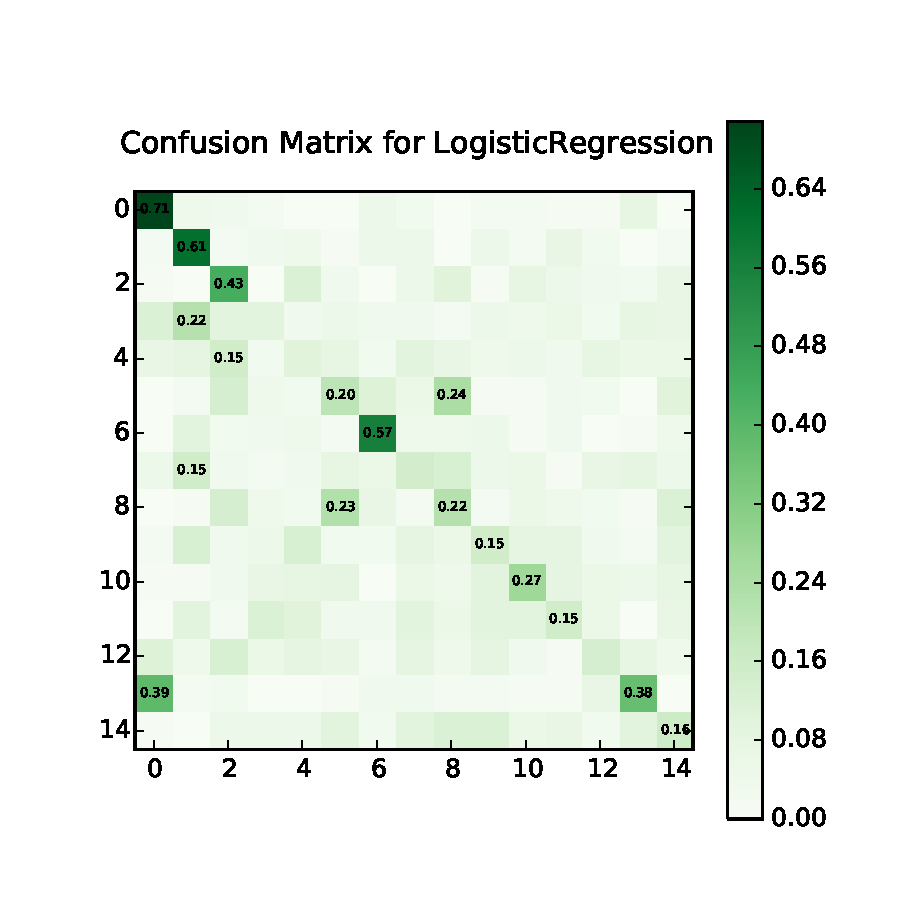
\includegraphics[width=\linewidth]{images/baseline/cm_log_reg.pdf}
		\caption{Logistic Regression Confusion Matrix Results}
	\end{subfigure}
	\hfill
	\begin{subfigure}[b]{0.45\linewidth}
		\centering
		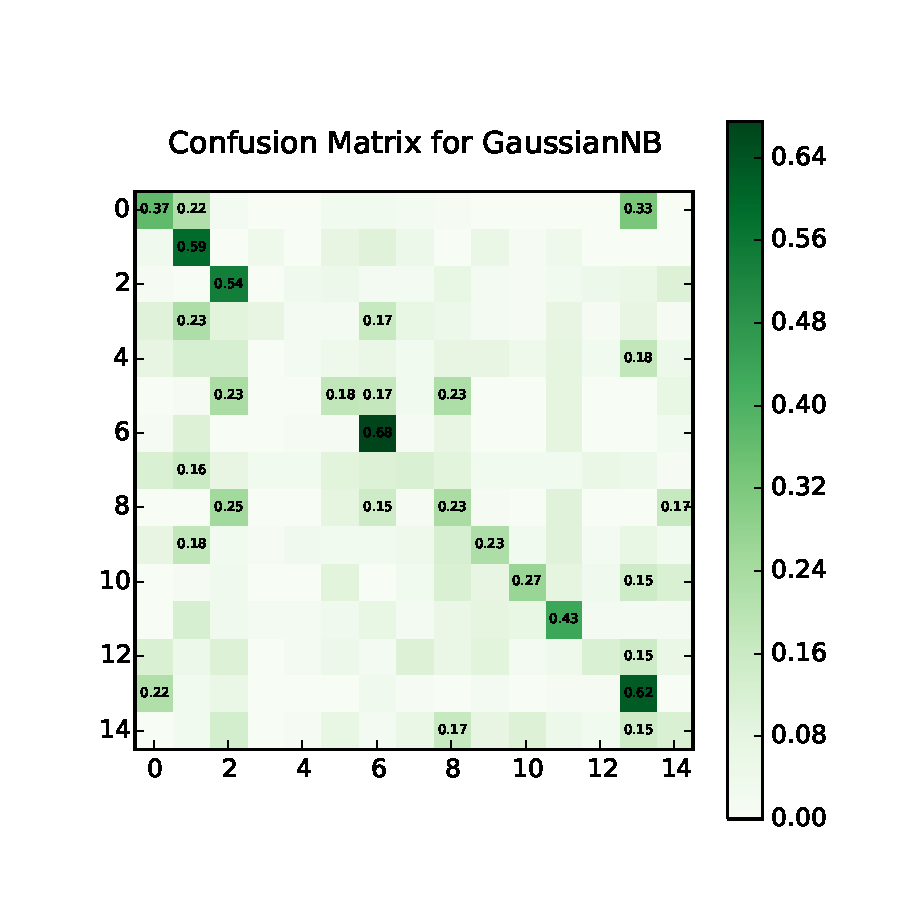
\includegraphics[width=\linewidth]{images/baseline/cm_naive_bayes.pdf}
		\caption{Gaussian Naive Bayes Confusion Matrix Results}
	\end{subfigure}
	\hfill
	\begin{subfigure}[b]{0.45\linewidth}
		\centering
		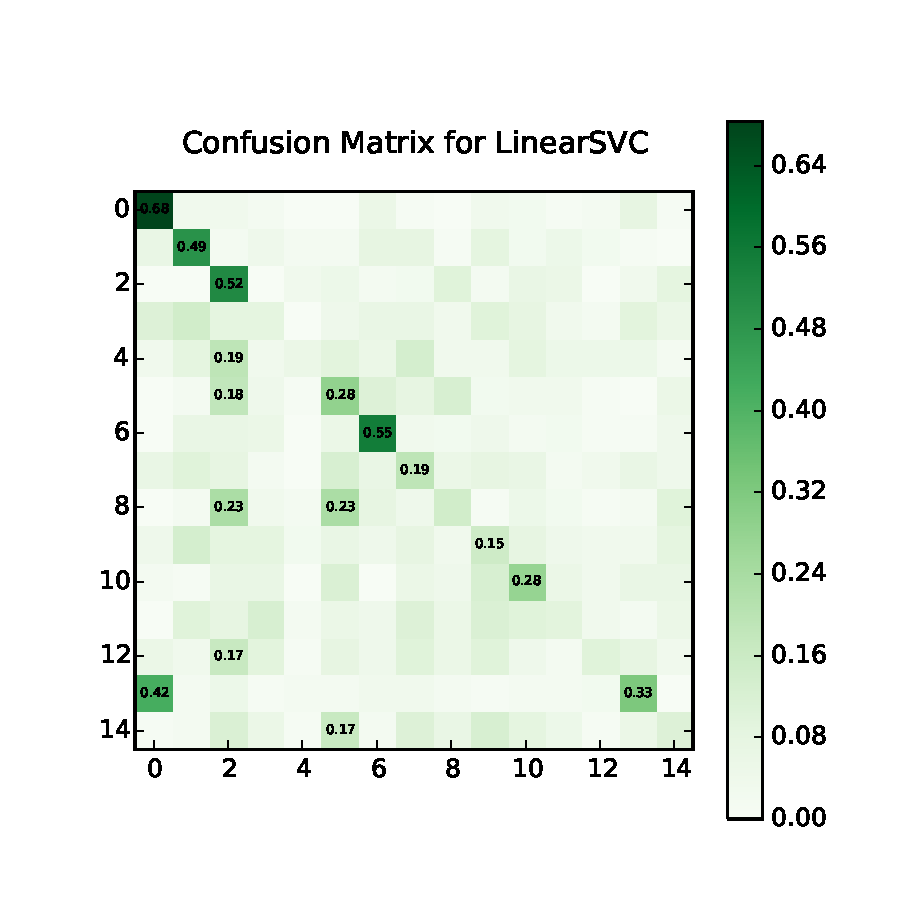
\includegraphics[width=\linewidth]{images/baseline/cm_linear_svm.pdf}
		\caption{Linear SVM Confusion Matrix Results}
	\end{subfigure}
	\hfill
	\begin{subfigure}[b]{0.45\linewidth}
		\centering
		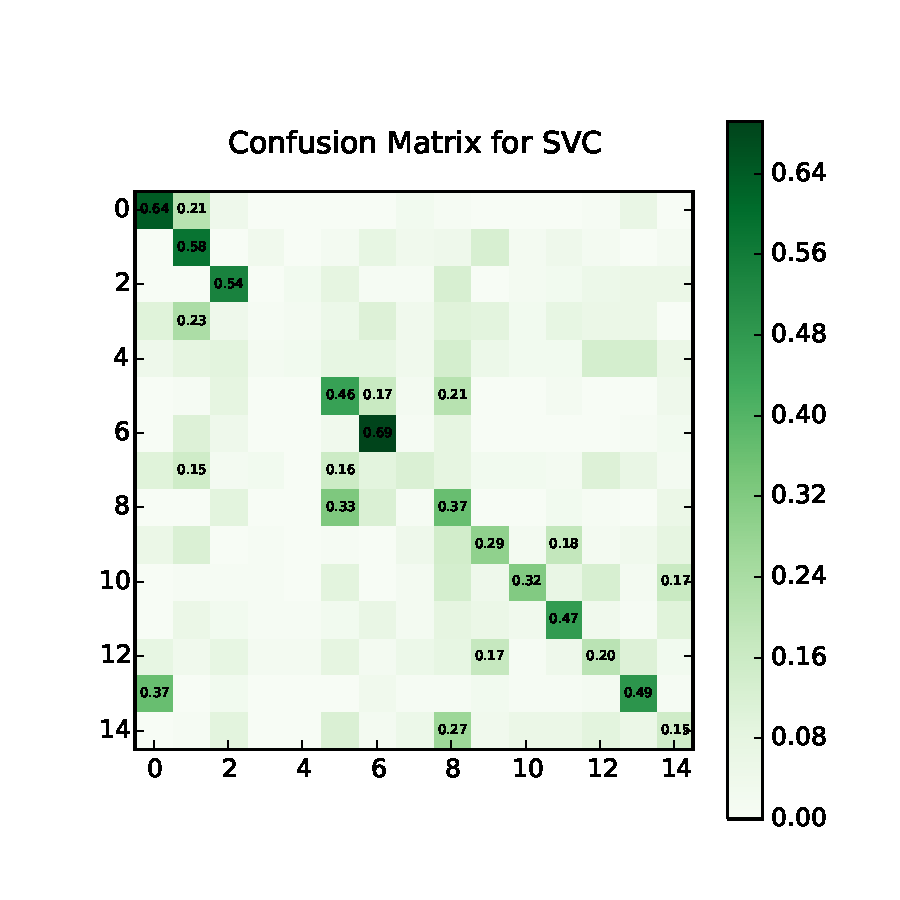
\includegraphics[width=\linewidth]{images/baseline/cm_svm.pdf}
		\caption{SVM Confusion Matrix Results}
	\end{subfigure}
	\caption{Confusion Matrices for the different baseline classifiers.}
	\label{baselines}
\end{figure}


\section{Neural Network Trained on LBP Results} \label{appendix:images}
\begin{figure}[H]
	\centering
	\begin{subfigure}[b]{0.45\linewidth}
		\centering
		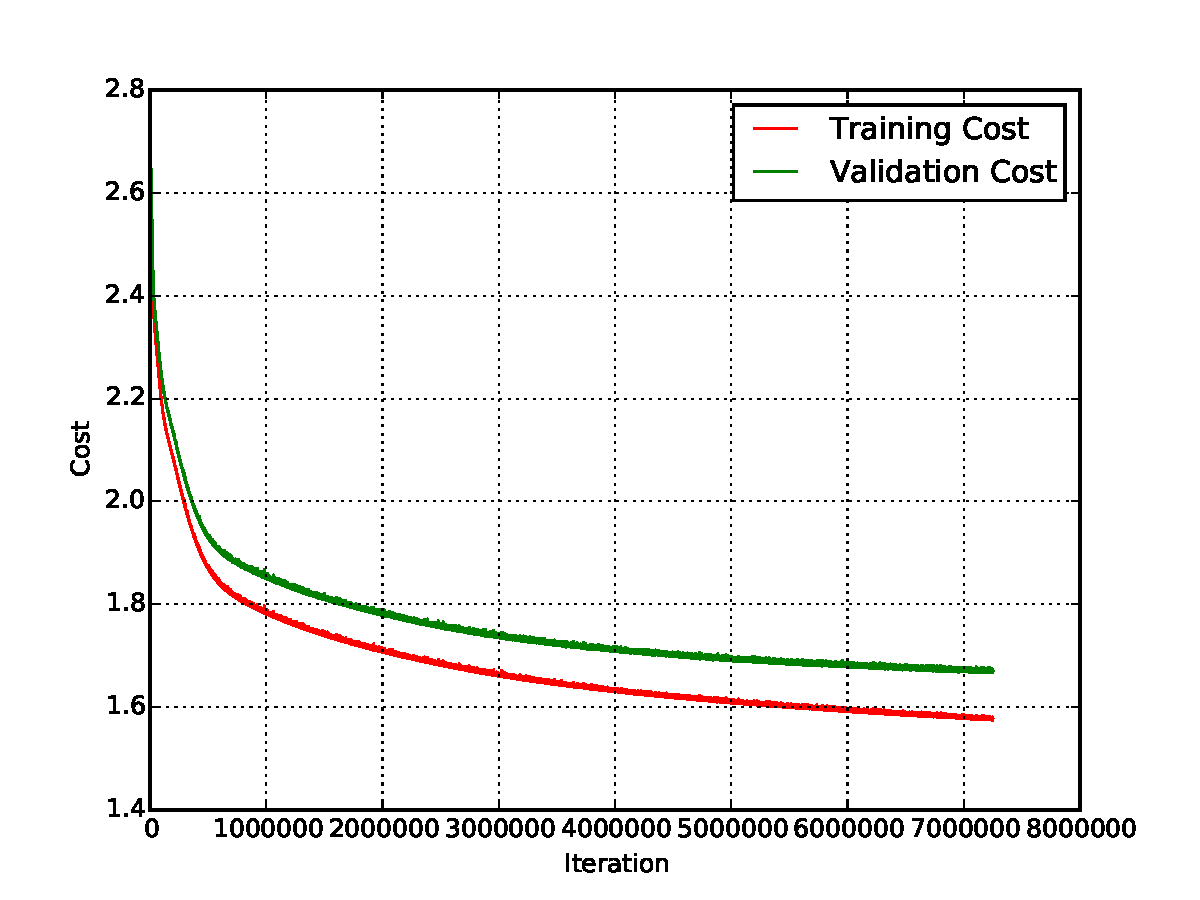
\includegraphics[width=\linewidth]{images/1/train_val_cost.pdf}
		\caption{Training versus Validation Cost}
	\end{subfigure}
	\hfill
	\begin{subfigure}[b]{0.45\linewidth}
		\centering
		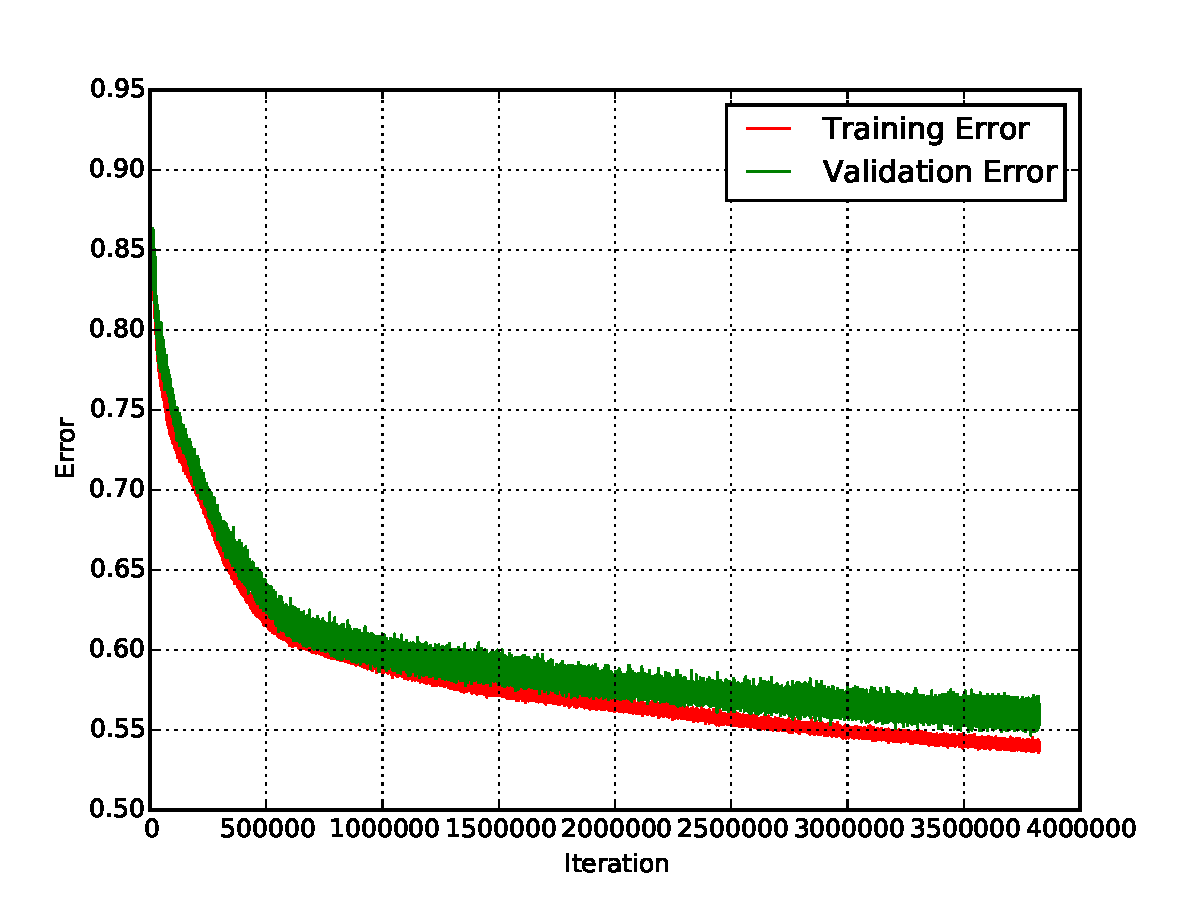
\includegraphics[width=\linewidth]{images/1/train_val_error.pdf}
		\caption{Training versus Validation Error}
	\end{subfigure}
	\caption{Learning curves for a feed-forward neural network with one hidden layer of 256 units trained on LBP.}
	\label{shrine1_curves}
\end{figure}
\begin{figure}[H]
	\centering
	\begin{subfigure}[b]{0.45\linewidth}
		\centering
		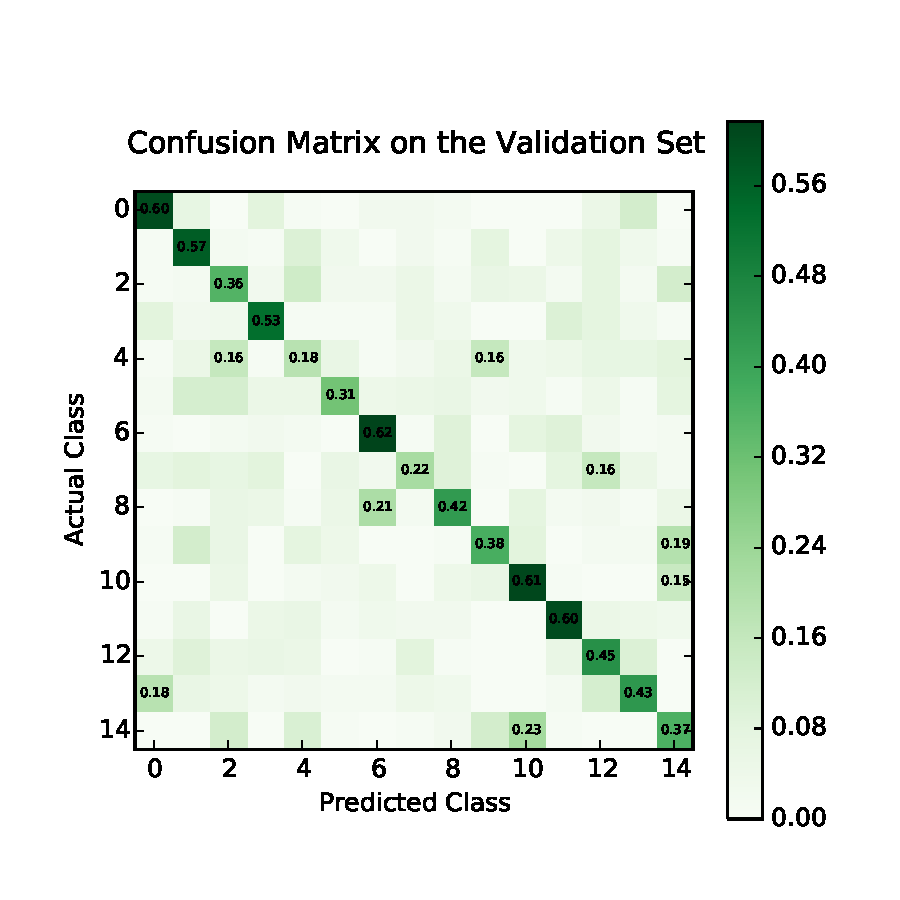
\includegraphics[width=\linewidth]{images/1/cm_valid.pdf}
		\caption{Confusion Matrix on the Validation Set}
	\end{subfigure}
	\hfill
	\begin{subfigure}[b]{0.45\linewidth}
		\centering
		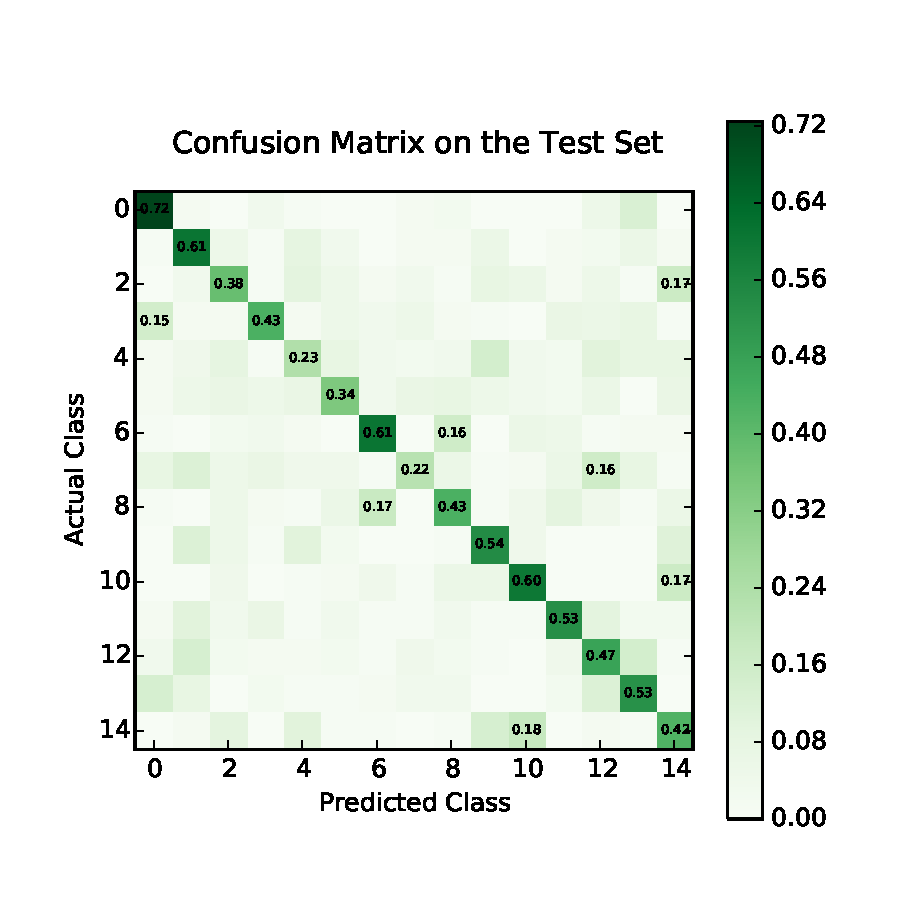
\includegraphics[width=\linewidth]{images/1/cm_test.pdf}
		\caption{Confusion Matrix on the Test Set}
	\end{subfigure}
	\caption{Confusion Matrices for a feed-forward neural network with one hidden layer of 256 unit trained on LBP.}
	\label{shrine1_mat}
\end{figure}

\begin{figure}
	\centering
	\begin{subfigure}[b]{0.45\linewidth}
		\centering
		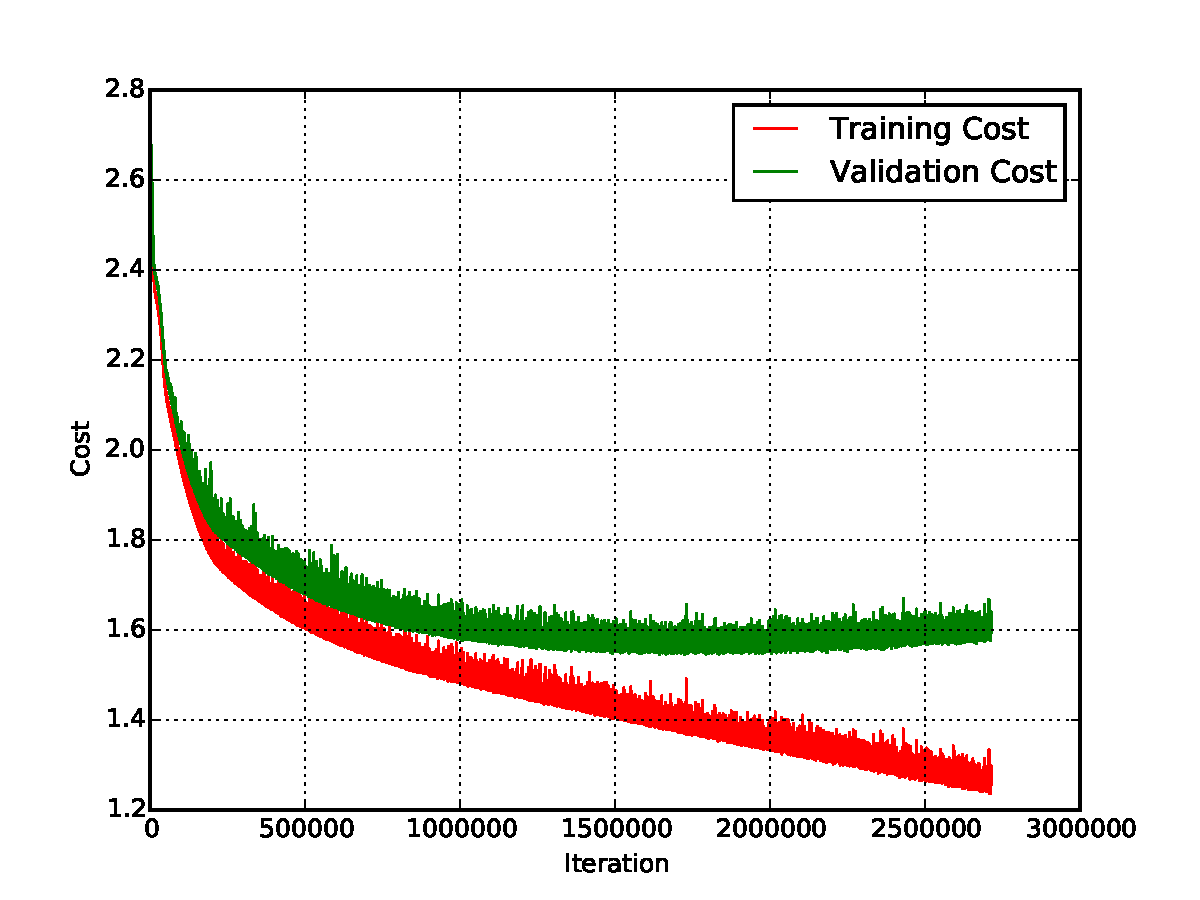
\includegraphics[width=\linewidth]{images/0/train_val_cost.pdf}
		\caption{Training versus Validation Cost}
	\end{subfigure}
	\hfill
	\begin{subfigure}[b]{0.45\linewidth}
		\centering
		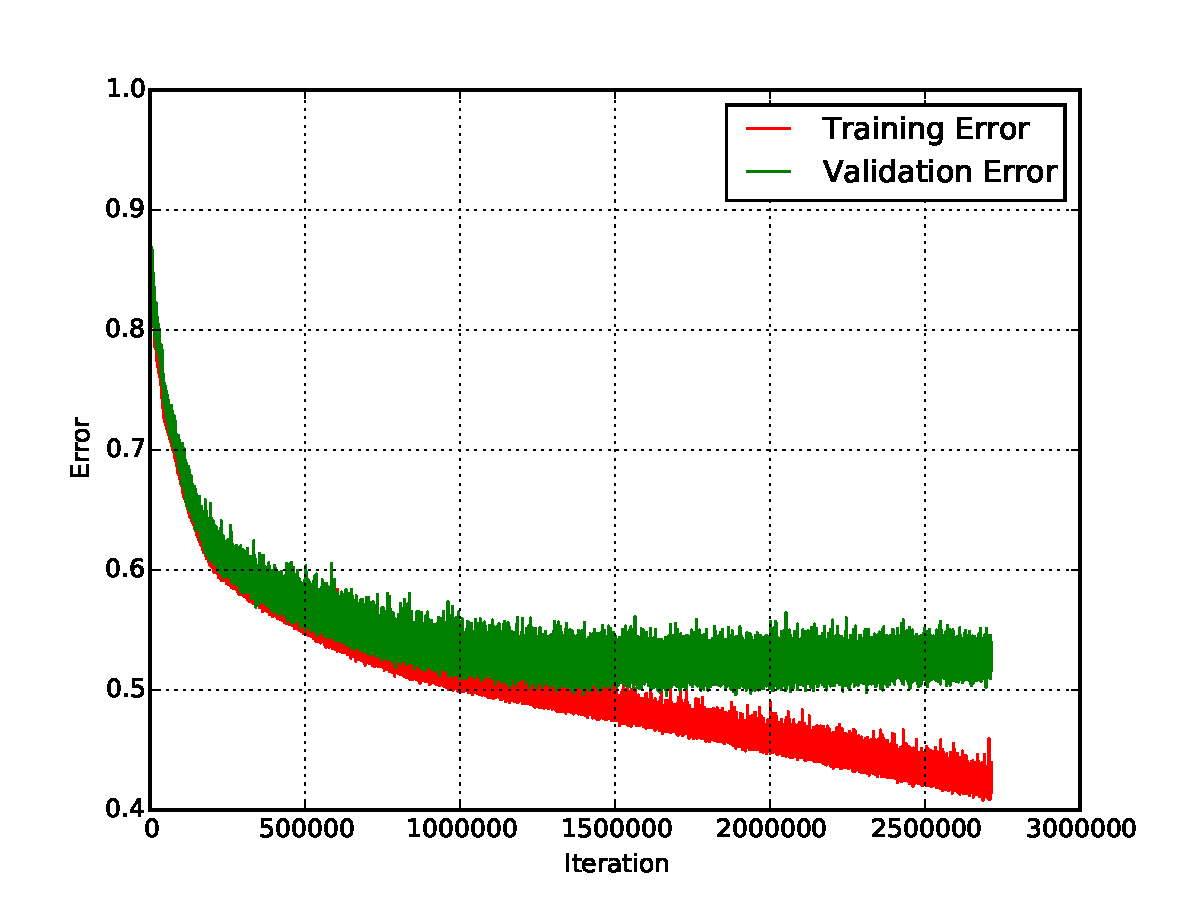
\includegraphics[width=\linewidth]{images/0/train_val_error.pdf}
		\caption{Training versus Validation Error}
	\end{subfigure}
	\caption{Learning curves for a feed-forward neural network with two hidden layers of 256 units each trained on LBP.}
	\label{shrine0_curves}
\end{figure}
\begin{figure}
	\centering
	\begin{subfigure}[b]{0.45\linewidth}
		\centering
		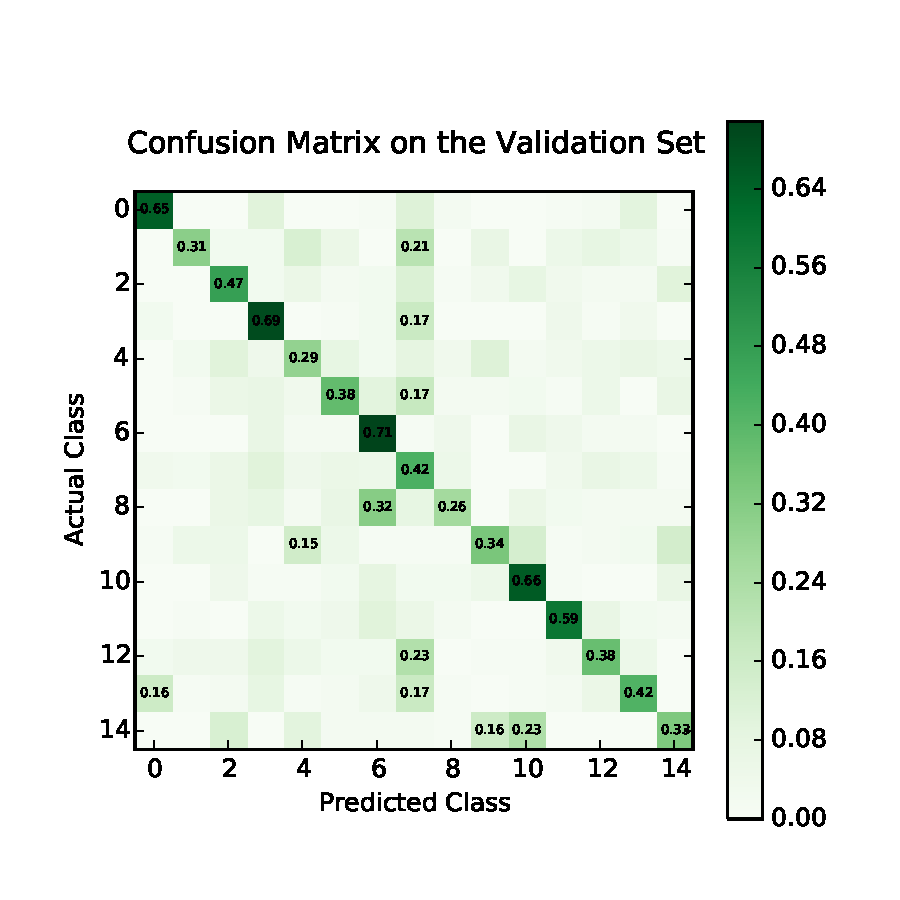
\includegraphics[width=\linewidth]{images/0/cm_valid.pdf}
		\caption{Confusion Matrix on the Validation Set}
	\end{subfigure}
	\hfill
	\begin{subfigure}[b]{0.45\linewidth}
		\centering
		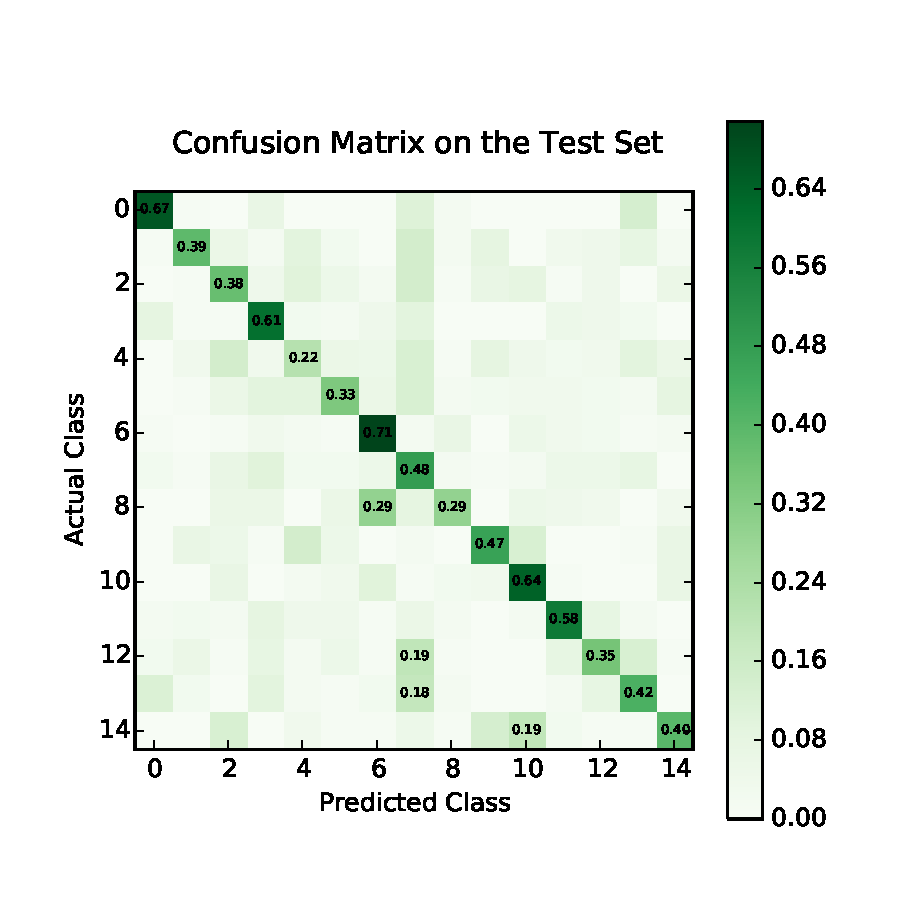
\includegraphics[width=\linewidth]{images/0/cm_test.pdf}
		\caption{Confusion Matrix on the Test Set}
	\end{subfigure}
	\caption{Confusion Matrices for a feed-forward neural network with two hidden layers of 256 units each trained on LBP.}
	\label{shrine0_mat}
\end{figure}

\begin{figure*}
	\centering
	\begin{subfigure}[b]{0.45\linewidth}
		\centering
		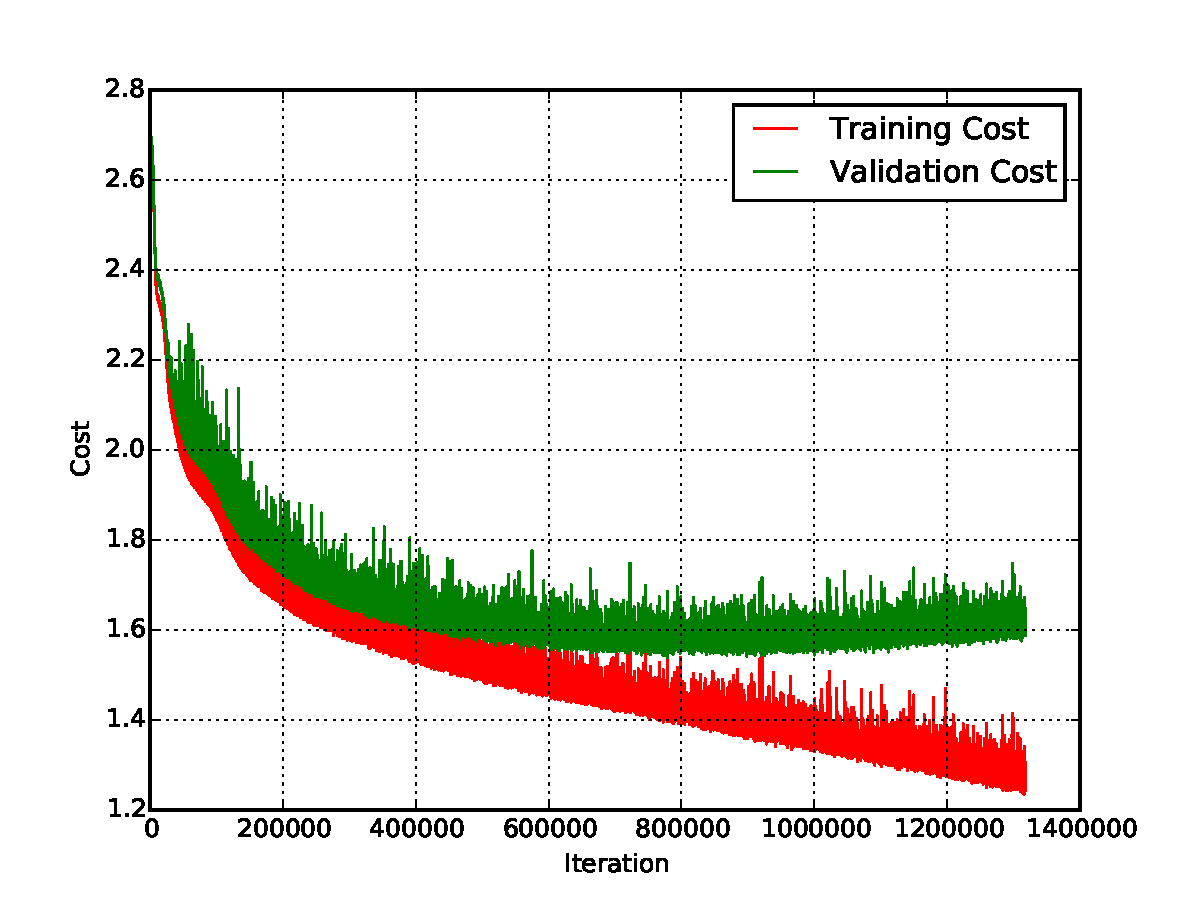
\includegraphics[width=\linewidth]{images/2/train_val_cost.pdf}
		\caption{Training versus Validation Cost}
	\end{subfigure}
	\hfill
	\begin{subfigure}[b]{0.45\linewidth}
		\centering
		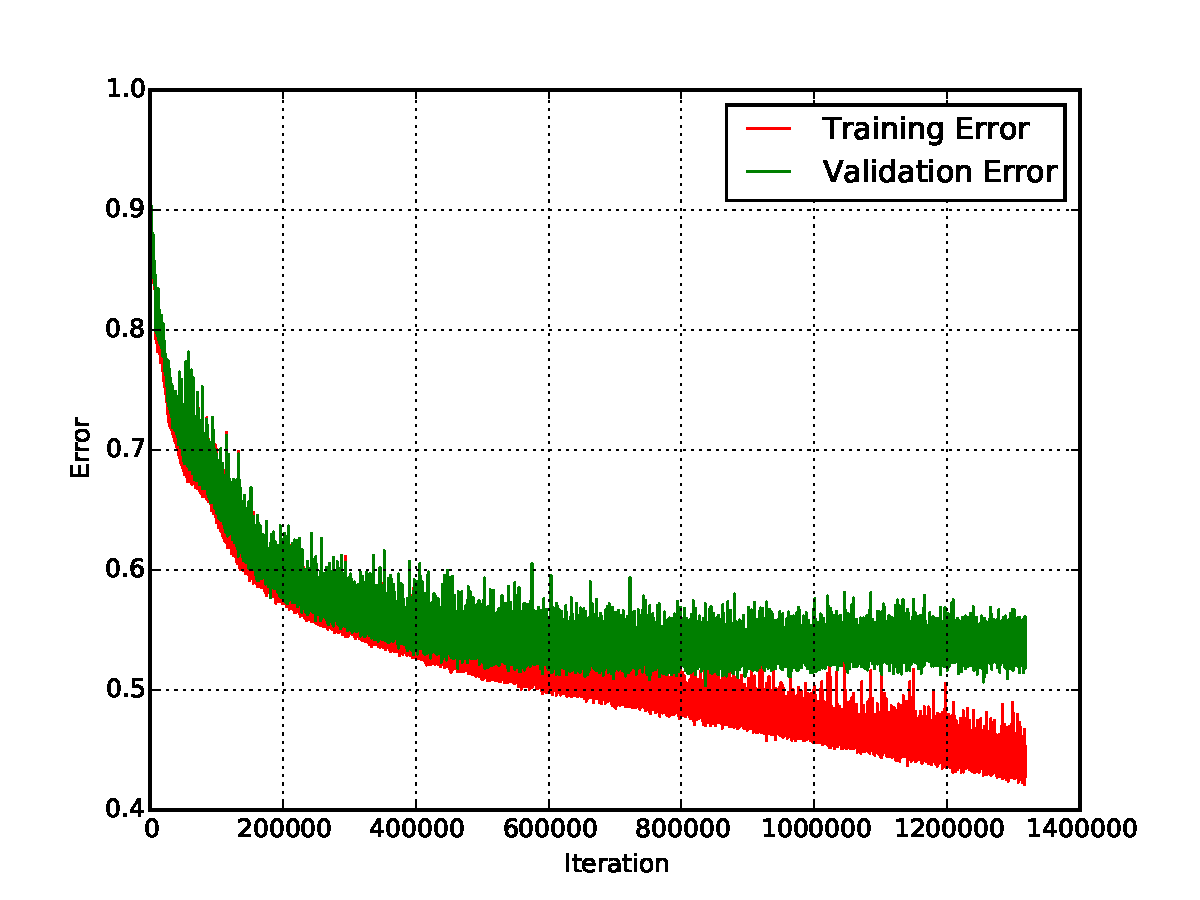
\includegraphics[width=\linewidth]{images/2/train_val_error.pdf}
		\caption{Training versus Validation Error}
	\end{subfigure}
	\caption{Learning curves for a feed-forward neural network with three hidden layers of 256, 128, 64 units.} 
	\label{shrine2_curves}
\end{figure*}
\begin{figure*}
	\centering
	\begin{subfigure}[b]{0.45\linewidth}
		\centering
		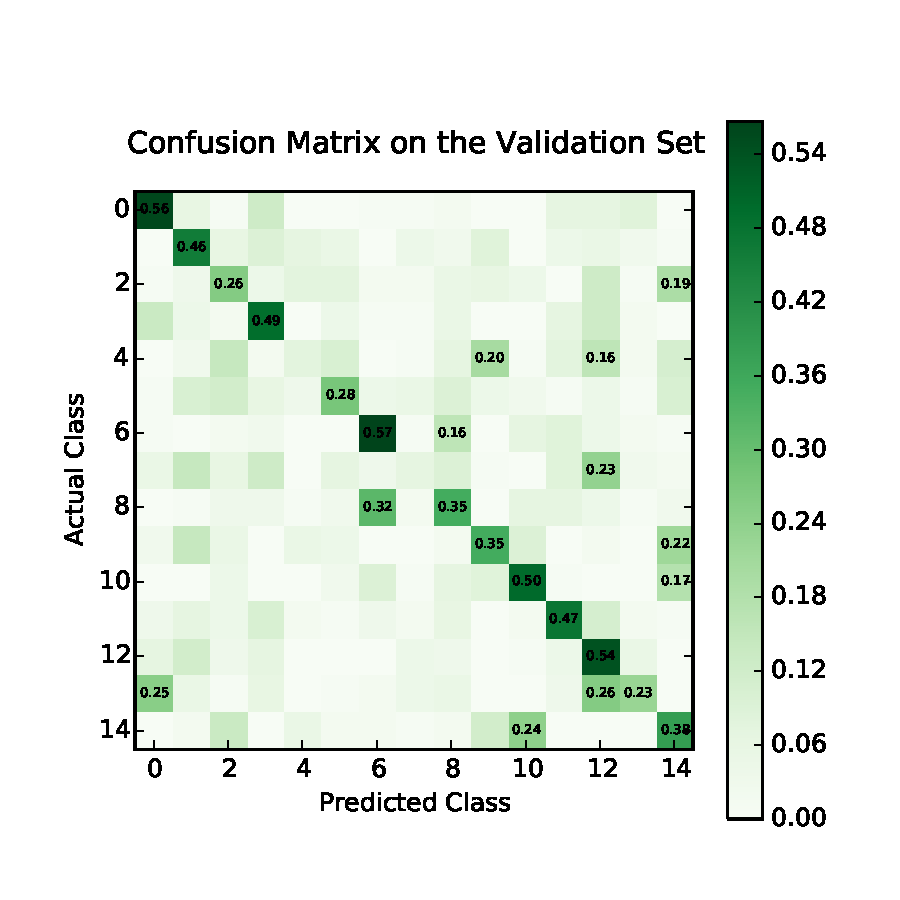
\includegraphics[width=\linewidth]{images/2/cm_valid.pdf}
		\caption{Confusion Matrix on the Validation Set}
	\end{subfigure}
	\hfill
	\begin{subfigure}[b]{0.45\linewidth}
		\centering
		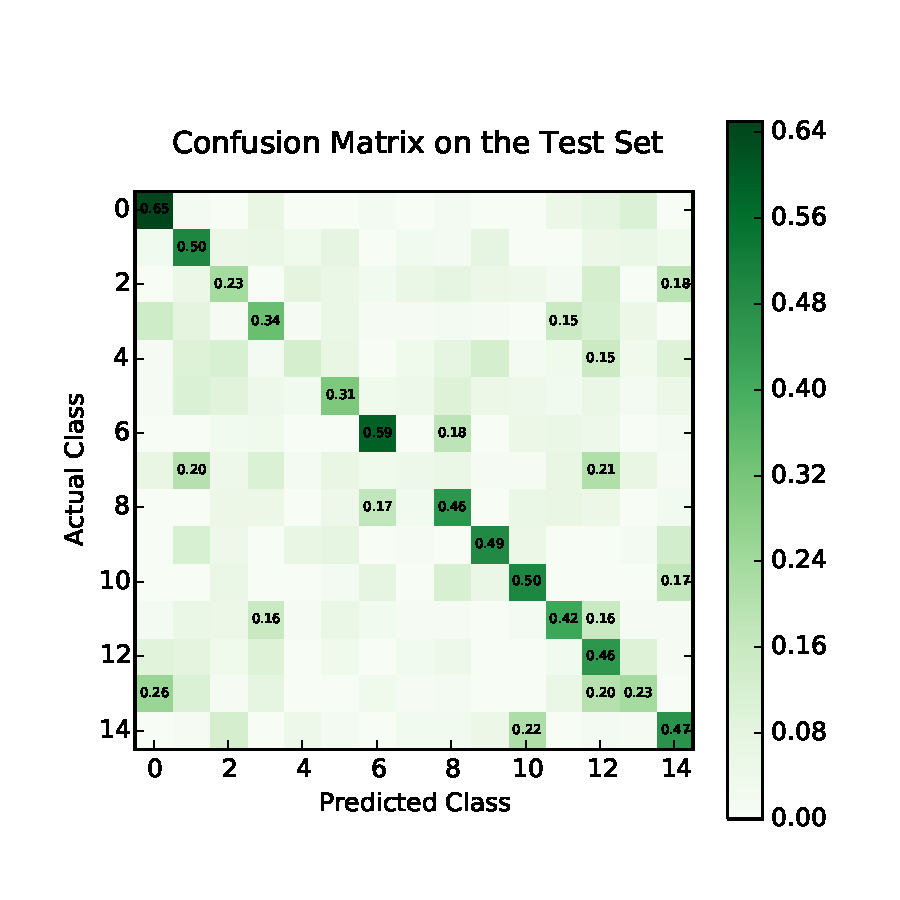
\includegraphics[width=\linewidth]{images/2/cm_test.pdf}
		\caption{Confusion Matrix on the Test Set}
	\end{subfigure}
	\caption{Confusion Matrices for a feed-forward neural network with three hidden layers of 256, 128, 64 units.}
	\label{shrine2_mat}
\end{figure*}


\section{Convolutional Neural Network Results}
\begin{figure}[H]
	\centering
	\begin{subfigure}[b]{0.45\linewidth}
		\centering
		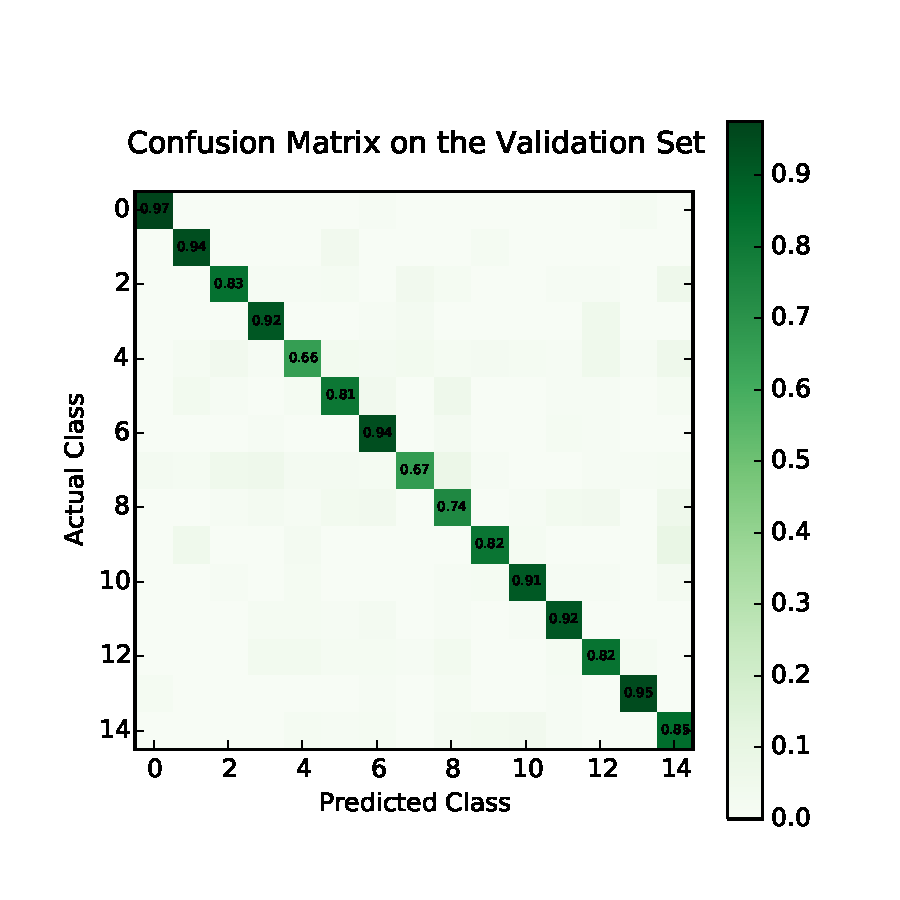
\includegraphics[width=\linewidth]{images/3/cm_valid.pdf}
		\caption{Confusion Matrix on the Validation Set}
	\end{subfigure}
	\hfill
	\begin{subfigure}[b]{0.45\linewidth}
		\centering
		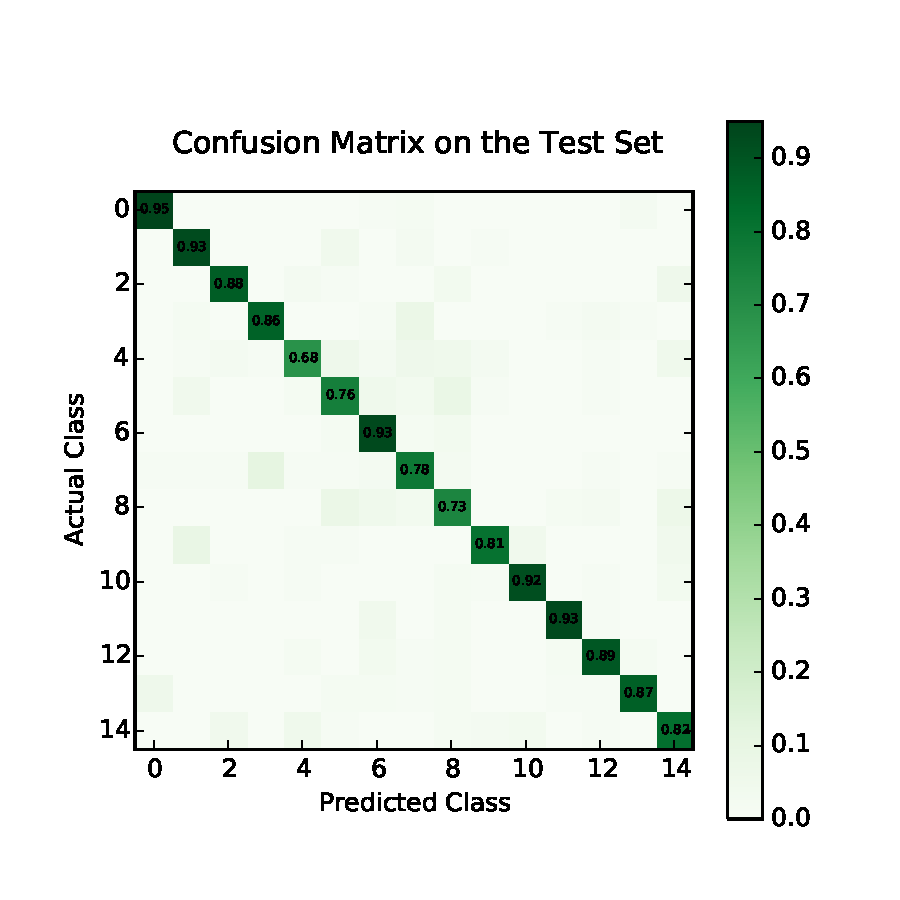
\includegraphics[width=\linewidth]{images/3/cm_test.pdf}
		\caption{Confusion Matrix on the Test Set}
	\end{subfigure}
	\caption{Confusion Matrices of our Convolutional Neural Network with three convolutional layers}
	\label{cnn_cm}
\end{figure}

\begin{figure}[H]
	\centering
	\begin{subfigure}[b]{0.45\linewidth}
		\centering
		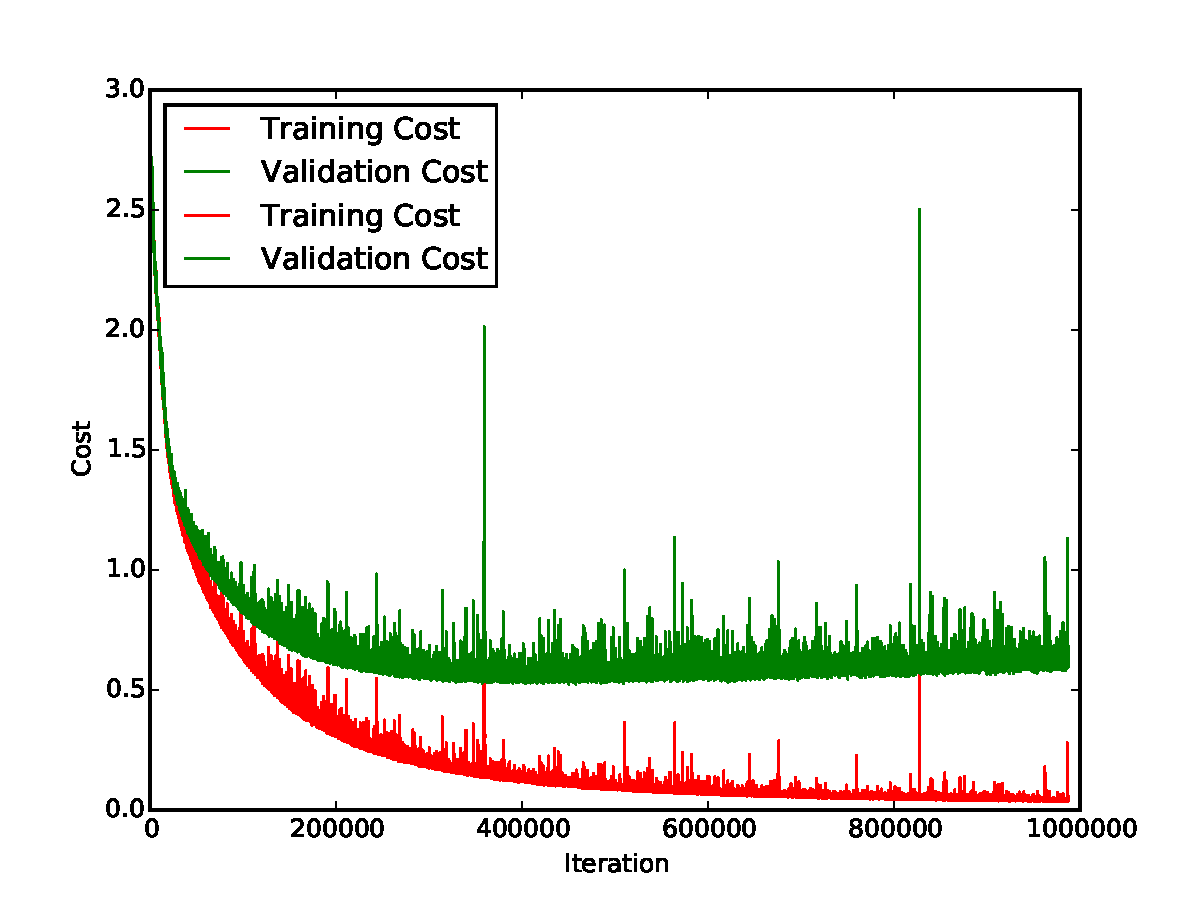
\includegraphics[width=\linewidth]{images/3/train_val_cost.pdf}
		\caption{Training versus Validation Cost}
	\end{subfigure}
	\hfill
	\begin{subfigure}[b]{0.45\linewidth}
		\centering
		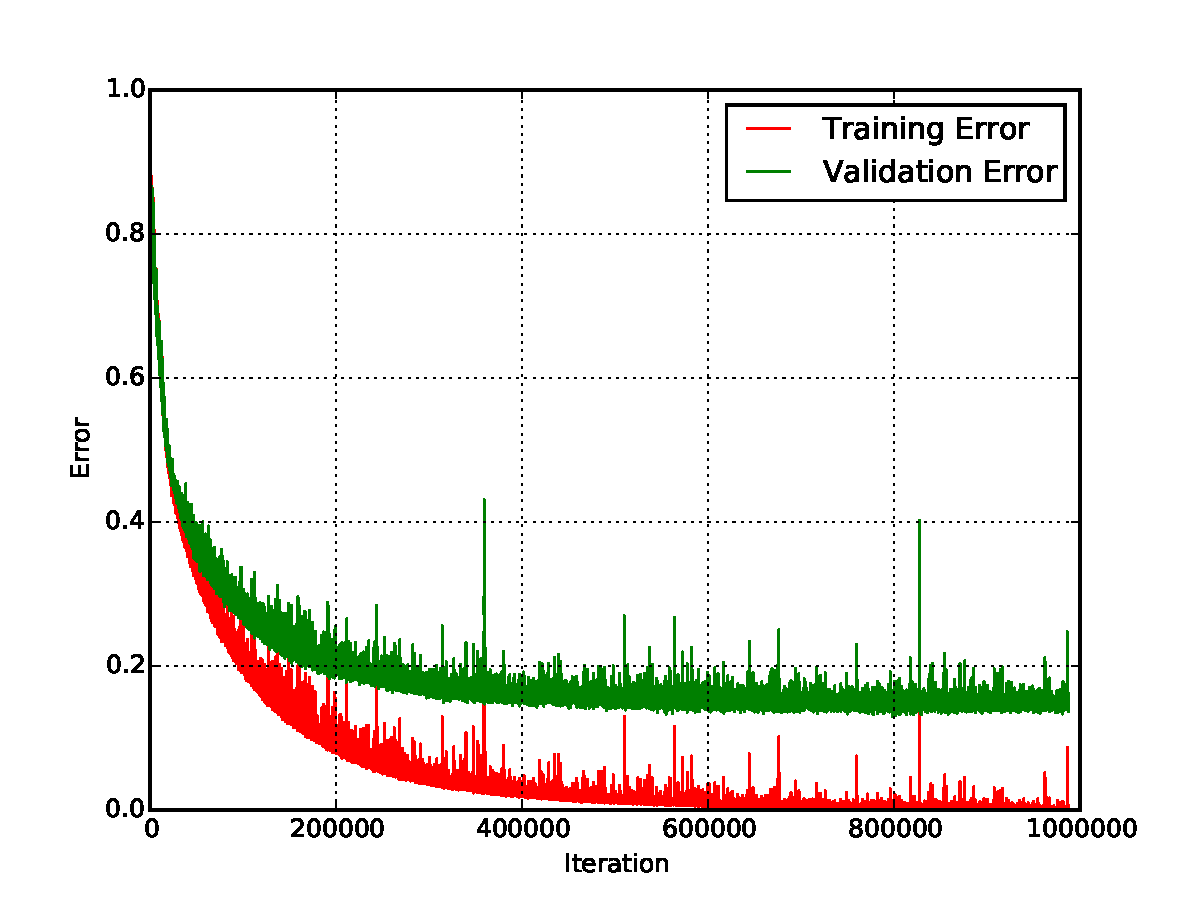
\includegraphics[width=\linewidth]{images/3/train_val_error.pdf}
		\caption{Training versus Validation Error}
	\end{subfigure}
	\caption{Learning curves for our Convolutional Neural Network with three hidden layers }
	\label{cnn_plot}
\end{figure}


\newpage
\begin{multicols}{2}
\paragraph*{} \lettrine[nindent=0em,lines=1]{\textit{W}}{}\textit{e hereby state that all the work presented in this report is that of the authors. }
\paragraph*{} Alan wrote the sections for \emph{Related Work} and \emph{Neural Network Approach}. Alan programmed the feed-forward neural network in \texttt{emerald.py} and extracted the Local Binary Patterns from the dataset in \texttt{purify\_dataset.py}. 
\par Kian created the rotated dataset and wrote its section \emph{Transformed Dataset}, programmed the baseline learners and wrote the content for \emph{Baseline Results} and \emph{Conclusion}. 
\par Genevieve wrote the \emph{Introduction}, \emph{Problem Definition} sections, and the results and discussion of CNN.
\par Genevieve and Kian programmed the CNN with help from Alan's \texttt{emerald.py}. 
\bibliography{ref}
\bibliographystyle{plainnat}
\end{multicols}
\end{document}
